\documentclass[12pt,a4paper,titlepage]{article}

\usepackage{textcomp} %I don't know why it needs this
\usepackage{titlesec} %spacing for sections
\usepackage[utf8]{inputenc}	% Unicode support
\usepackage[margin=0.5in]{geometry}
\usepackage[pdftex]{graphicx}% Picture handling
	\graphicspath{{./Tests/}}
	\DeclareGraphicsExtensions{.pdf,.jpeg,.png}
\usepackage{epstopdf}
\usepackage{tocloft}		% Table Of Contents

\usepackage{color}			%colors
	\definecolor{light-gray}{gray}{0.92}
	
\usepackage{listings}		% Formatting and highlighting
	\lstset{
	basicstyle=\footnotesize,
	breaklines=true,
    tabsize=2,
    framextopmargin=50pt,
    rulecolor=\color{black},
    backgroundcolor=\color{light-gray}
    }
\usepackage{hyperref}		% linking to other sections


\author{Stefano Dalla Longa\\pID 10535602 \and Nicolò Brandolese\\pID 10531144}
\date{}
\title{Prova Finale di Reti Logiche, AA 2019-2020}


\begin{document}
	%title page
	\begin{titlepage}
    \begin{center}
        \vspace*{3cm}
            
        \Huge
        \textbf{Prova Finale di Reti Logiche}
            
        \vspace{0.5cm}
        \LARGE
        AA. 2019/2020
            
        \vspace{1.5cm}
            
        \textbf{Stefano Dalla Longa, pID 10535602 \\ Nicolò Brandolese, pID 10531144}
        
        \vspace{1.2 cm}
        \Large
		Politecnico di Milano, scaglione prof. Fornaciari
            
        \vspace{0.8cm}
            
    \end{center}
\end{titlepage}

	\renewcommand{\contentsname}{Indice}	%renaming table of contents

	\tableofcontents
	\clearpage	%using \newpage gives a wrong table of content enumeration
	\section{Introduzione}
   
		Abbiamo deciso di risolvere questo problema in maniera sequenziale: provando ogni \textit{working zone}\footnote{Da ora in poi, spesso ci si riferirà alle working zone con la dicitura "WZ"} presente una alla volta e riportando un risultato positivo al primo successo oppure un risultato negativo dopo l'ottavo fallimento.
In questo modo l'implementazione è scalabile ad un (teorico) infinito numero di WZ diverse con minimale aumento di volume; a pagarne le conseguenze sono le prestazioni nel caso pessimo (indirizzo appartenente all'ultima WZ o non appartenente a nessuna WZ), ma, data la natura del problema di utilizzo delle working zone, si assume che il caso pessimo sia poco frequente.
Per ulteriori speculazioni sulle performance della soluzione implementata, si guardi la sezione \hyperref[sec:ottimizzazione]{\textit{5.3: Limitazioni e possibili ottimizzazioni - ottimizzazione dei dati nella RAM}}.
       
	\section{Descrizione della macchina e dei processi}
		L'implementazione si basa sulla scomposizione in quattro sottoproblemi:
		\begin{enumerate}
			\item comunicazione con la RAM per la lettura dei dati
			\item computazione per determinare l'appartenenza dell'indirizzo base ad una working zone
			\item gestione del flusso d'esecuzione in base al risultato della computazione
			\item comunicazione con la RAM per la scrittura del risultato
		\end{enumerate}
		La scelta di risoluzione è stata la creazione di una macchina a stati finiti, in particolare una macchina di Mealy, basata su tre macroprocessi:
		\begin{itemize}
			%state register
			\item \textit{\texttt{state\_register}}: ad ogni fronte di salita del clock propaga il valore del prossimo stato della macchina \textit{\texttt{next\_state}} al registro dello stato corrente \textit{\texttt{current\_state}}. Reagisce al segnale di reset eseguendo un reset sincrono, ovvero assegnando invece il valore di \textit{\texttt{START\_IDLE}} a \textit{\texttt{current\_state}} sul fronte di salita del clock;
			
			%speak with ram
			\item \textit{\texttt{speak\_with\_RAM}}: gestisce i valori dei segnali in input e output, ad eccezione di \textit{\texttt{o\_done}} il quale è gestito da \textit{\texttt{calc\_process}};
			
			%calc process
			\item \textit{\texttt{calc\_process}}: esegue i calcoli per determinare se l'indirizzo base appartiene alla working zone considerata;
		\end{itemize}
		
		ai quali si aggiungono tre ulteriori processi dedicati alla gestione degli elementi di memoria interni:
		\begin{itemize}
			%segnale di reset
			\item \textit{\texttt{reset\_handler}}: tiene traccia della richiesta di reset da parte della RAM tramite il segnale in input \textit{\texttt{i\_rst}} e permette di eseguire un reset sincrono. Si veda la sezione \hyperref[sec:reset]{\textit{5.2: Limitazioni e possibili ottimizzazioni - segnale di reset}} per ulteriori chiarimenti sul funzionamento della procedura di reset.	
			
			%contatore delle working zone
			\item \textit{\texttt{wz\_counter\_process}}: aggiorna sul fronte di discesa del clock il contatore \textit{\texttt{wz\_counter}} delle working zone già controllate. Il contenuto di tale contatore è aggiornato ad ogni nuova esecuzione della macchina, ed è dotato di segnale di reset. L'aggiornamento sul fronte di discesa anziché di salita del clock risolve diversi problemi di sincronia tra il contatore e i successivi stati, dal momento che il suo valore deve essere disponibile allo stato immediatamente successivo all'aggiornamento del suo contenuto.
			
			%gestione dei flip-flop edge-triggered
			\item \textit{\texttt{FF\_saving}}: gestisce i flip-flop relativi a quattro segnali da memorizzare. Non è stato necessario fornirlo di segnale di reset.
			
		\end{itemize}
		
		Una rappresentazione schematica della macchina è fornita dalla figura seguente:
		\begin{center}
			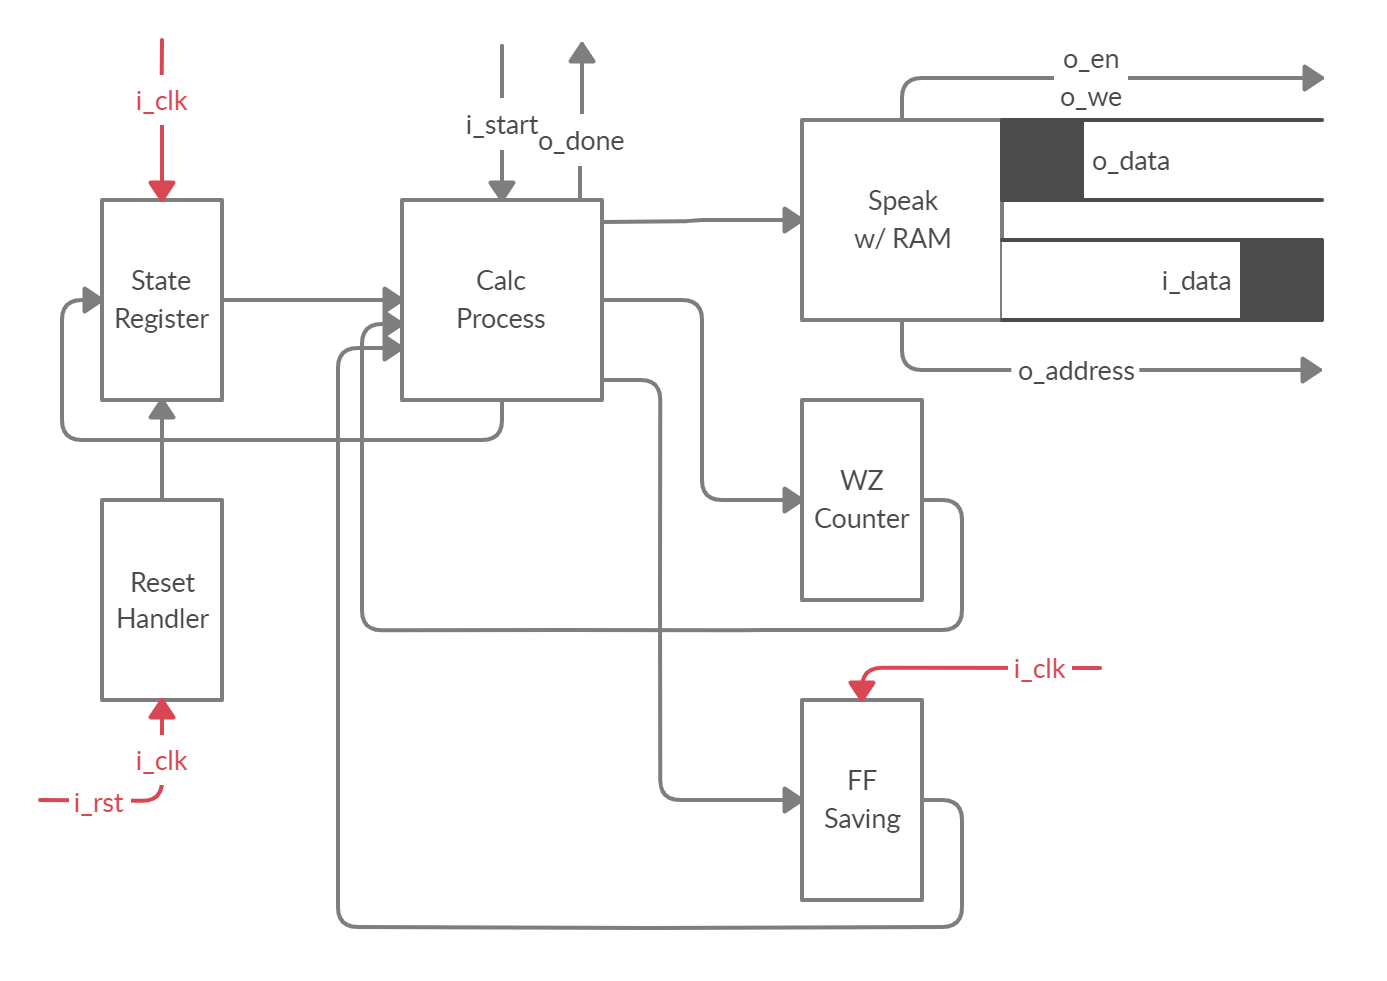
\includegraphics[scale=0.325]{arch_v1_1.png}
		\end{center}
		
		Abbiamo scelto di separare \textit{\texttt{calc\_process}} e \textit{\texttt{speak\_with\_RAM}} per ragioni di leggibilità, dal momento che da un punto di vista teorico entrambi costituiscono una componente combinatoria della stessa macchina a stati finiti, e perciò sarebbe stato possibile accorparli nel medesimo processo. Dal momento però che VHDL proibisce di modificare lo stesso segnale da processi diversi, la gestione del flusso modificando il valore di \textit{\texttt{next\_state}} è affidata esclusivamente a \textit{\texttt{calc\_process}}.

		\section{Descrizione degli stati}
		Il flusso d'esecuzione e la transizione dello stato corrente della macchina sono schematizzati nella figura seguente e usano questa convenzione:
		\begin{itemize}
		
		\item gli stati in blu sono tutti e soli gli stati nei quali opera \textit{\texttt{speak\_with\_RAM}} e sono progettati per durare un ciclo di clock;
		
		\item gli stati in verde sono gli stati di calcolo e codifica da parte di \textit{\texttt{calc\_process}}, anch'essi progettati per cambiare ad ogni ciclo di clock;
		
		\item gli stati in rosso sono stati di idle gestiti da \textit{\texttt{calc\_process}}, progettati per arrestare il flusso di esecuzione ed eventualmente ricominciare la computazione in base al valore di \textit{\texttt{i\_start}}.
		 \end{itemize}

		\begin{center}
			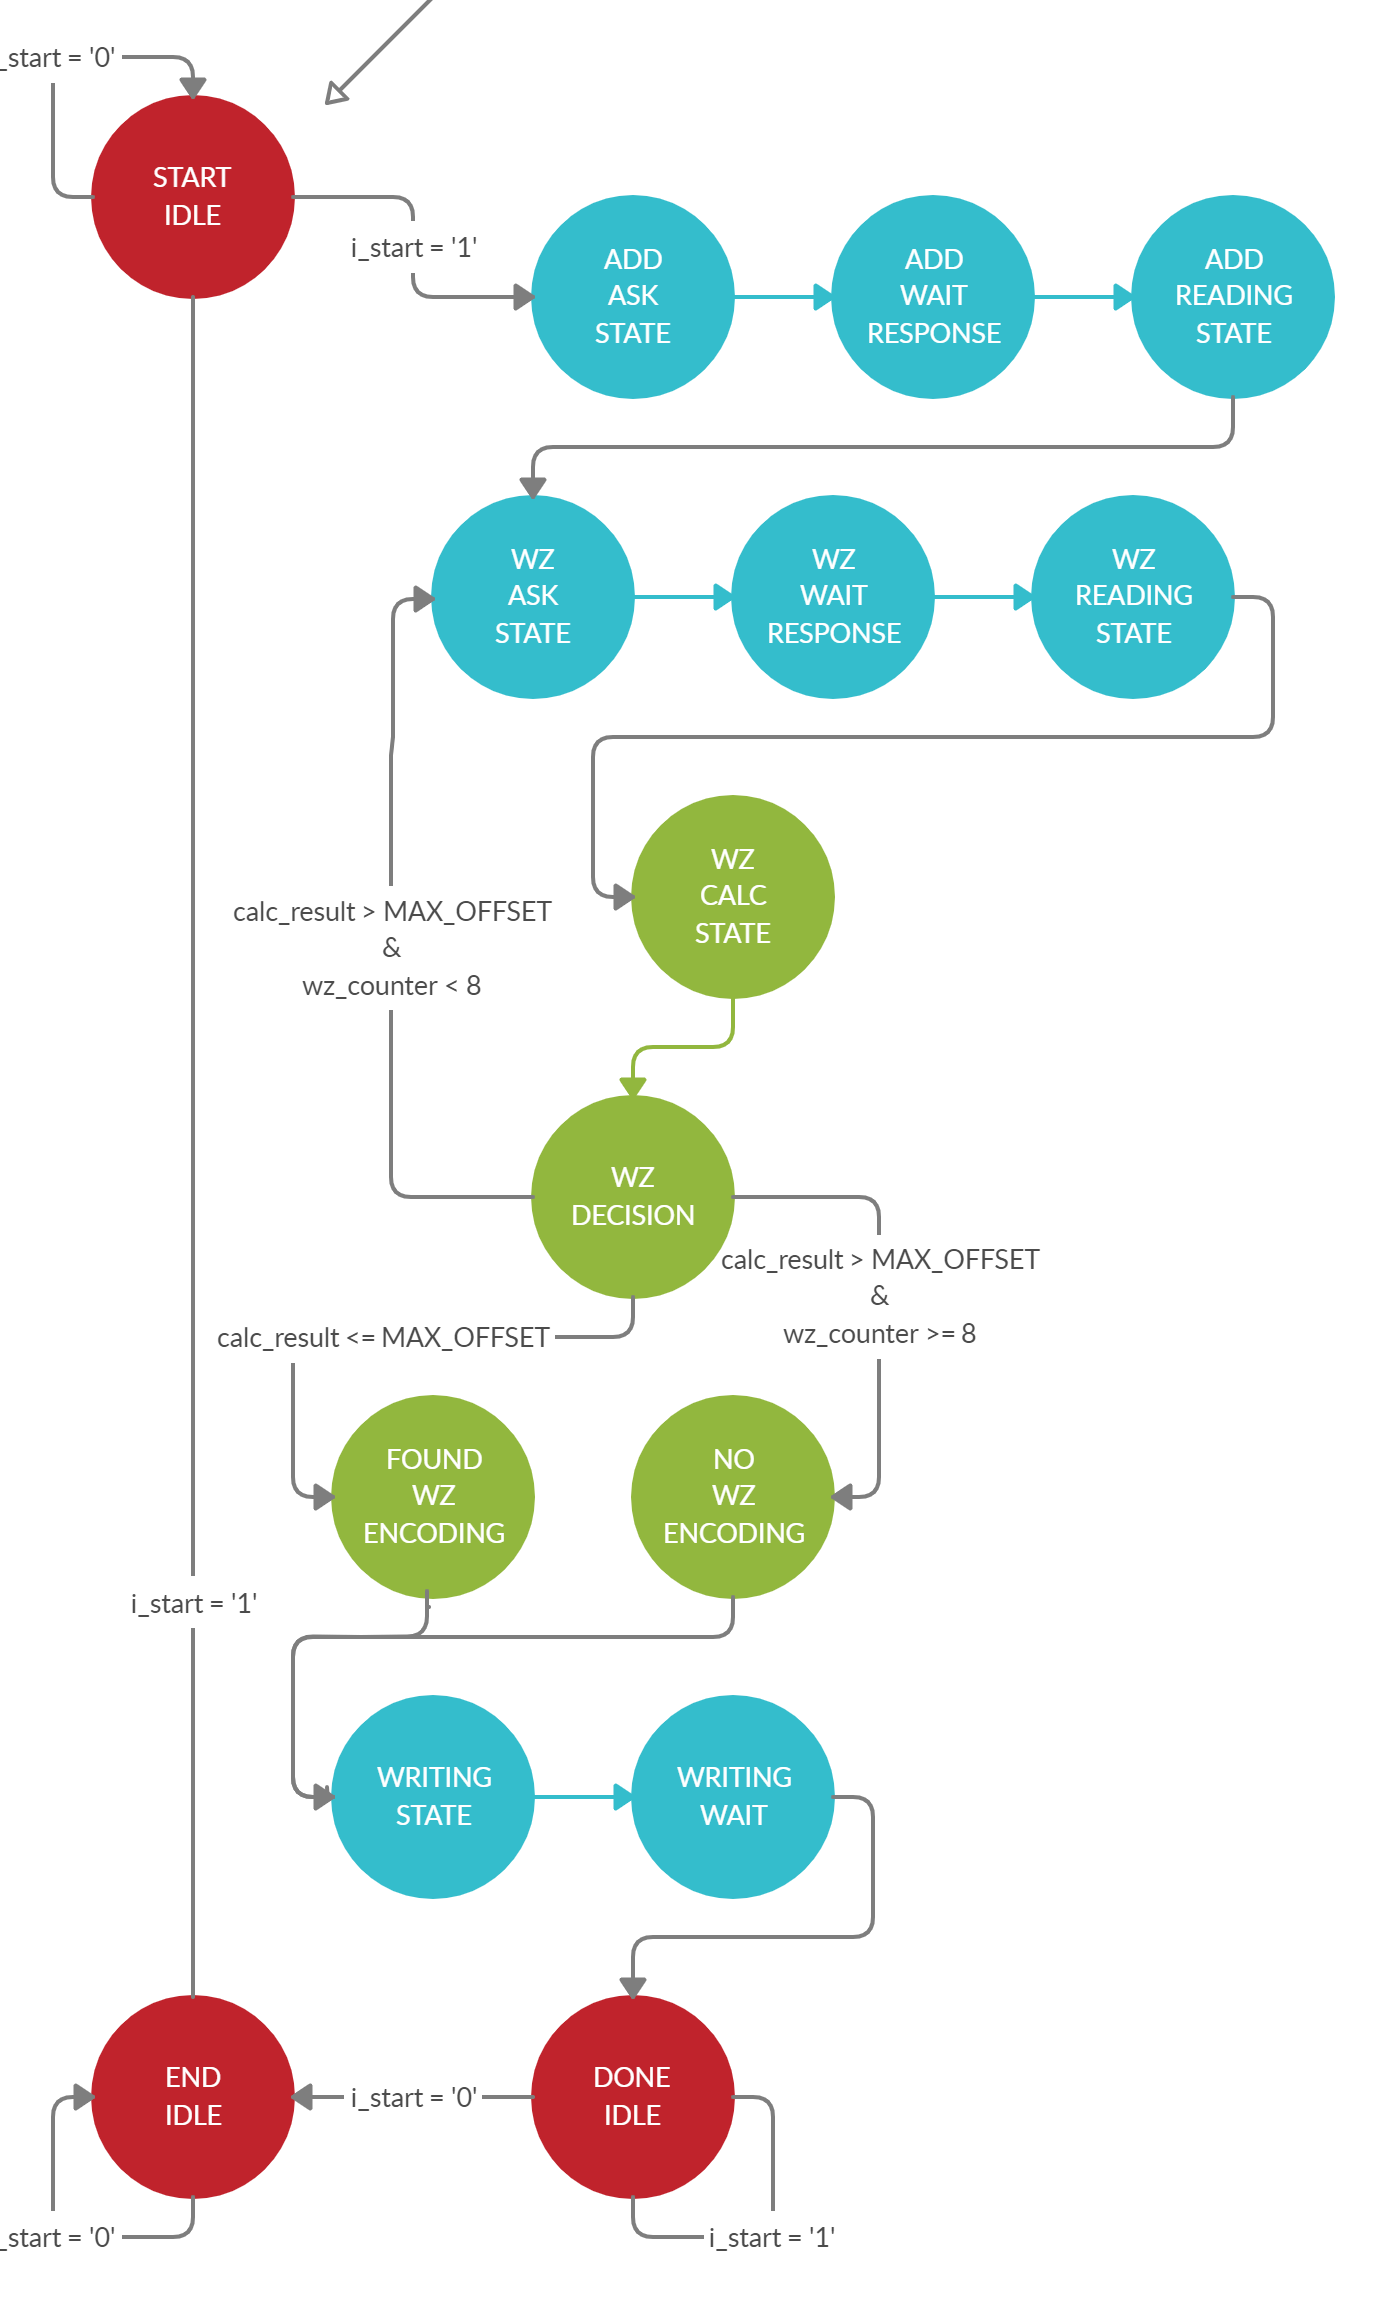
\includegraphics[scale=0.275]{retlog_FSM_v1_4.png}
		\end{center}
		
		Un breve riassunto del funzionamento di ogni stato è il seguente:
		
		\renewcommand{\descriptionlabel}[1]{\hspace{\labelsep}\textit{#1}}
		\begin{description}
		\item[START\_IDLE:] stato iniziale. La macchina resta in questo stato finché \textit{\texttt{i\_start}} vale $0$ e vi ritorna quando riceve un segnale di reset;
		\item[ADD\_ASK\_STATE:]		richiede alla RAM l'indirizzo base;
		\item[ADD\_WAIT\_RESPONSE:]	stato di attesa per permettere alla RAM di processare la richiesta;
		\item[ADD\_READING\_STATE:]	salva il valore dell'indirizzo base ricevuto in input dalla RAM nel registro
									\textit{\texttt{base\_address}};
		\item[WZ\_ASK\_STATE:]			richiede alla RAM l'$n$-esima working zone, dove $n$ è il valore del registro contatore
									\textit{\texttt{wz\_counter}};
		\item[WZ\_WAIT\_RESPONSE:]		stato di attesa per permettere alla RAM di processare la richiesta;
		\item[WZ\_READING\_STATE:]		salva il valore dell'$n$-esima working zone ricevuta in input dalla RAM nel registro
									\textit{\texttt{wz\_address}};
		\item[WZ\_CALC\_STATE:]		calcola se l'indirizzo base appartiene alla working zone corrente, con l'operazione tra registri $\textit{\texttt{calc\_result}} = \textit{\texttt{base\_address}} - \textit{\texttt{wz\_address}}$;
		\item[WZ\_DECISION:]		in base al valore di \textit{\texttt{calc\_result}}  in grado di capire se l'indirizzo base appartiene alla working zone considerata. In caso affermativo, imposta come prossimo stato \textit{\texttt{FOUND\_WZ\_ENCODING}}, mentre in caso contrario imposta come prossimo stato \textit{\texttt{NO\_WZ\_ENCODING}} se la working zone considerata era l'ultima contenuta nella RAM, oppure ritorna nello stato \textit{\texttt{WZ\_ASK\_STATE}} se la RAM contiene altre working zone da controllare\footnote{Quest'operazione costituisce il critical path della rete combinatoria};
		
		\item[FOUND\_WZ\_ENCODING:]	codifica la parola da scrivere nella ram nel registro \textit{\texttt{encoded\_res}} secondo 										la convenzione usata in caso di fallimento;
		\item[NO\_WZ\_ENCODING:]	codifica la parola da scrivere nella ram nel registro \textit{\texttt{encoded\_res}} secondo 										la convenzione usata in caso di successo;
		\item[WRITING\_STATE:]		scrive nella RAM il contenuto di \textit{\texttt{encoded\_res}};
		\item[WRITING\_WAIT:]		stato di attesa per permettere alla RAM di processare la richiesta;
		\item[DONE\_IDLE:]			notifica alla RAM la fine della computazione mantenendo al valore $1$ il segnale \textit{\texttt{o\_done}}. La macchina resta in questo stato finché il segnale \textit{\texttt{i\_start}} vale $1$, dopodiché va nello stato di \textit{\texttt{END\_IDLE}};
		\item[END\_IDLE:]			imposta a $0$ il segnale \textit{\texttt{o\_done}}. La macchina aspetta l'innalzamento del segnale \textit{\texttt{i\_start}}, in seguito al quale torna in \textit{\texttt{START\_IDLE}}.
		\end{description}
		
	\section{Test eseguiti} \label{sec:test}
       Per controllare il corretto funzionamento del circuito sono state svolte un centinaio di simulazioni, generate automaticamente (tranne pochi casi limite) e controllate manualmente. È stato usato uno script di python 3 per generare randomicamente il contenuto della RAM, scriverlo in un file di testo e scrivere il risultato da visualizzare in memoria, in codifica binaria, esadecimale e decimale, sotto forma di commento VHDL. È riportato il codice sorgente del programma, il quale accetta da riga di comando due elementi: il numero iniziale e il numero finale del test (riadattato per compatibilità con la nostra batteria di test).\newpage
       
	\begin{lstlisting}
	
import sys
import random

starting = int(sys.argv[1])	#starting element
ending = int(sys.argv[2])	#ending element

f = open("random_test.txt", "w")

for i in range(ending - starting + 1):
	addr_list = []
	f.write("\t\t\t\twhen %d =>\n\n" % (starting + i))
	
	for j in range(9):
		random_num = random.getrandbits(7)
		f.write("\t\t\t\tRAM(%d) " %(j))
		f.write("<= assign(%d);\n" %(random_num))
		addr_list.append(random_num)

	#expected value calculation
	f.write("\t\t\t\t--expected ")

	expected = addr_list[8]	#default value, in case the address doesn't belong to any working zone
	result = 0
	for l in range(len(addr_list)-1):
		found = 0
		result = expected - addr_list[l]
		if(result <= 3):	#found a suitable wz
			found = l
			break
	
	if(found != 0):		#you found a wz, now its bin encoding is written on file
		expected_bin = '1' + format(found, '03b') + (("0001" if result == 0 else "0010") if result <= 1 else ("0100" if result == 2 else "1000"))
		f.write(expected_bin[:4] + '.' + expected_bin[4:])
		f.write(' ')
		f.write(str(hex(int(expected_bin, 2)))[2:])
		f.write(' ')
		f.write(str(int(expected_bin, 2)))
		f.write('\n\n')
	else:
		expected_bin = format(expected, '08b')
		f.write(expected_bin[:4] + '.' + expected_bin[4:])	#expected is still the default value, which is now encoded into 8 digit binary number
		f.write(' ')
		f.write(str(hex(expected)[2:]))
		f.write(' ')
		f.write(str(expected))
		f.write('\n\n')

f.close()	#close file	
	
	\end{lstlisting}
	
	\newpage


Qui riportiamo i risultati dei quattro test per noi più importanti:

	\begin{enumerate}
	
	\item \textit{WZ in ordine crescente, risultato atteso negativo}: questo test si trova come esempio nella specifica
		\begin{center}
			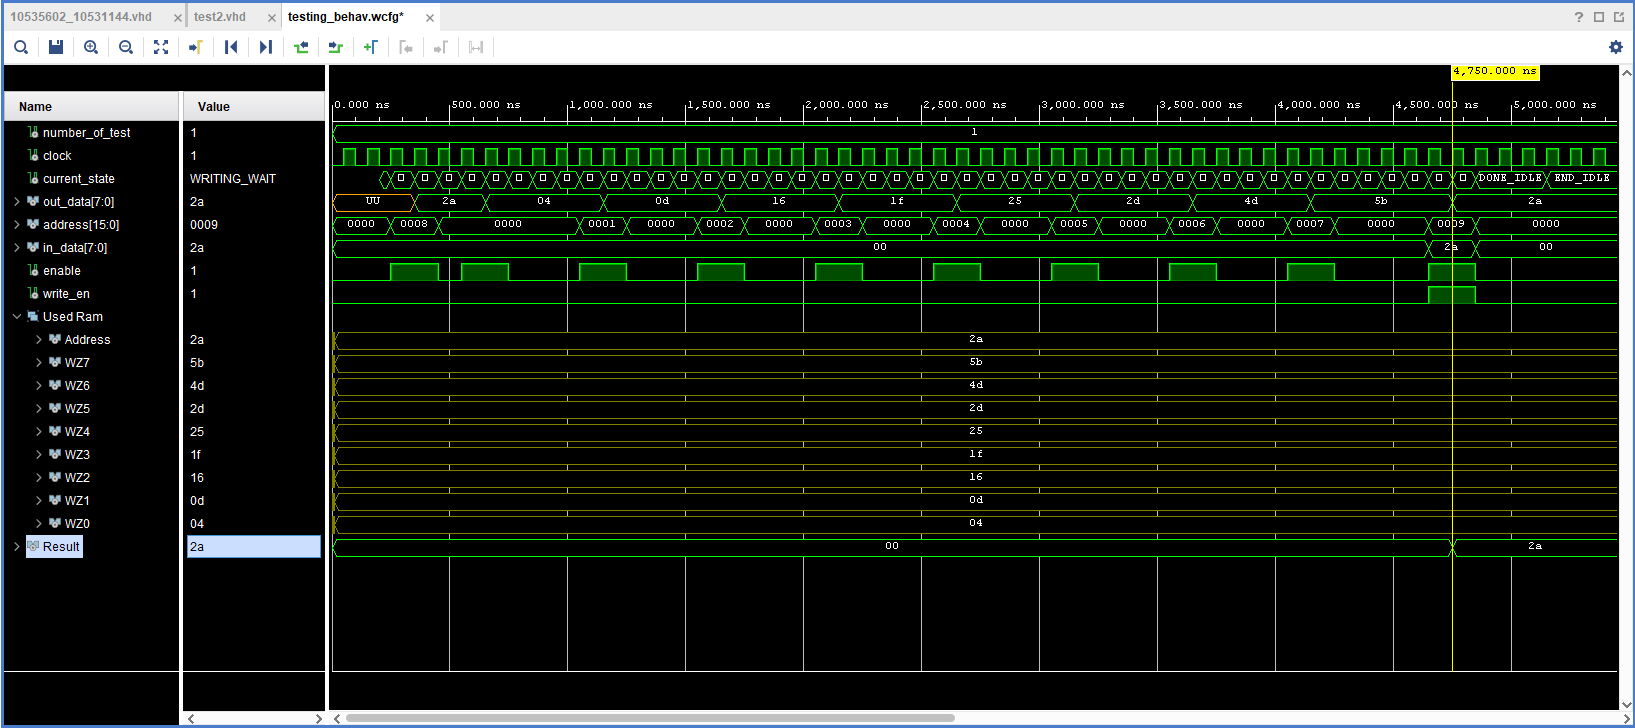
\includegraphics[scale=0.4]{test1.png}
		\end{center}
		%\vspace{0.5cm}
	
	\item \textit{WZ in ordine crescente, risultato atteso positivo}: questo test si trova come esempio nella specifica
	
		\begin{center}
			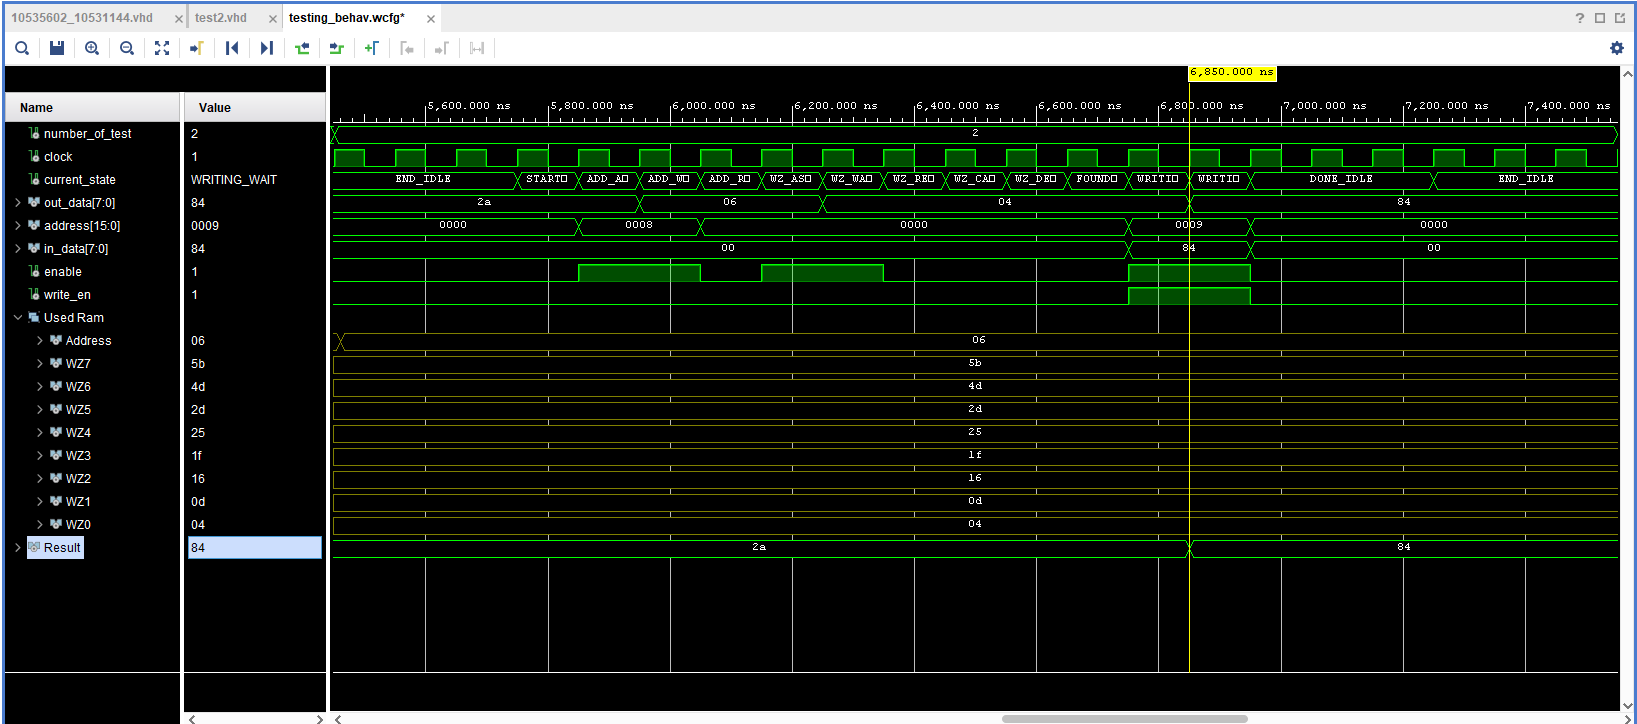
\includegraphics[scale=0.4]{test2.png}
		\end{center}
		%\vspace{0.5cm}

	\item \textit{WZ in ordine sparso, risultato atteso positivo}
	
		\begin{center}
			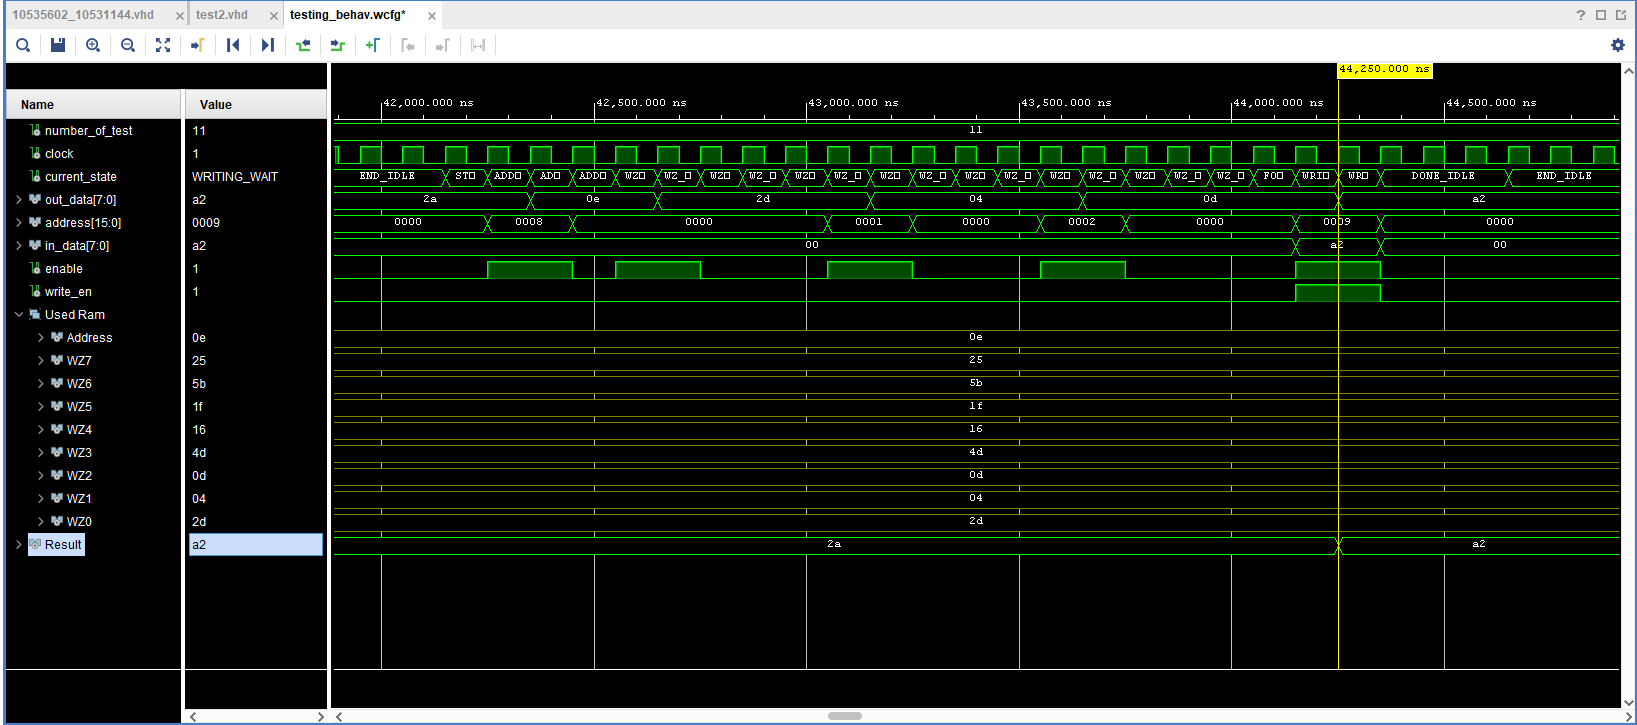
\includegraphics[scale=0.4]{test11.png}
		\end{center}
		%\vspace{0.5cm}

	\item \textit{WZ duplicate, risultato atteso positivo}: in questo caso viene considerato valido l'indirizzo della prima working zone che contiene l'indirizzo base, a prescindere dall'offset
	
		\begin{center}
			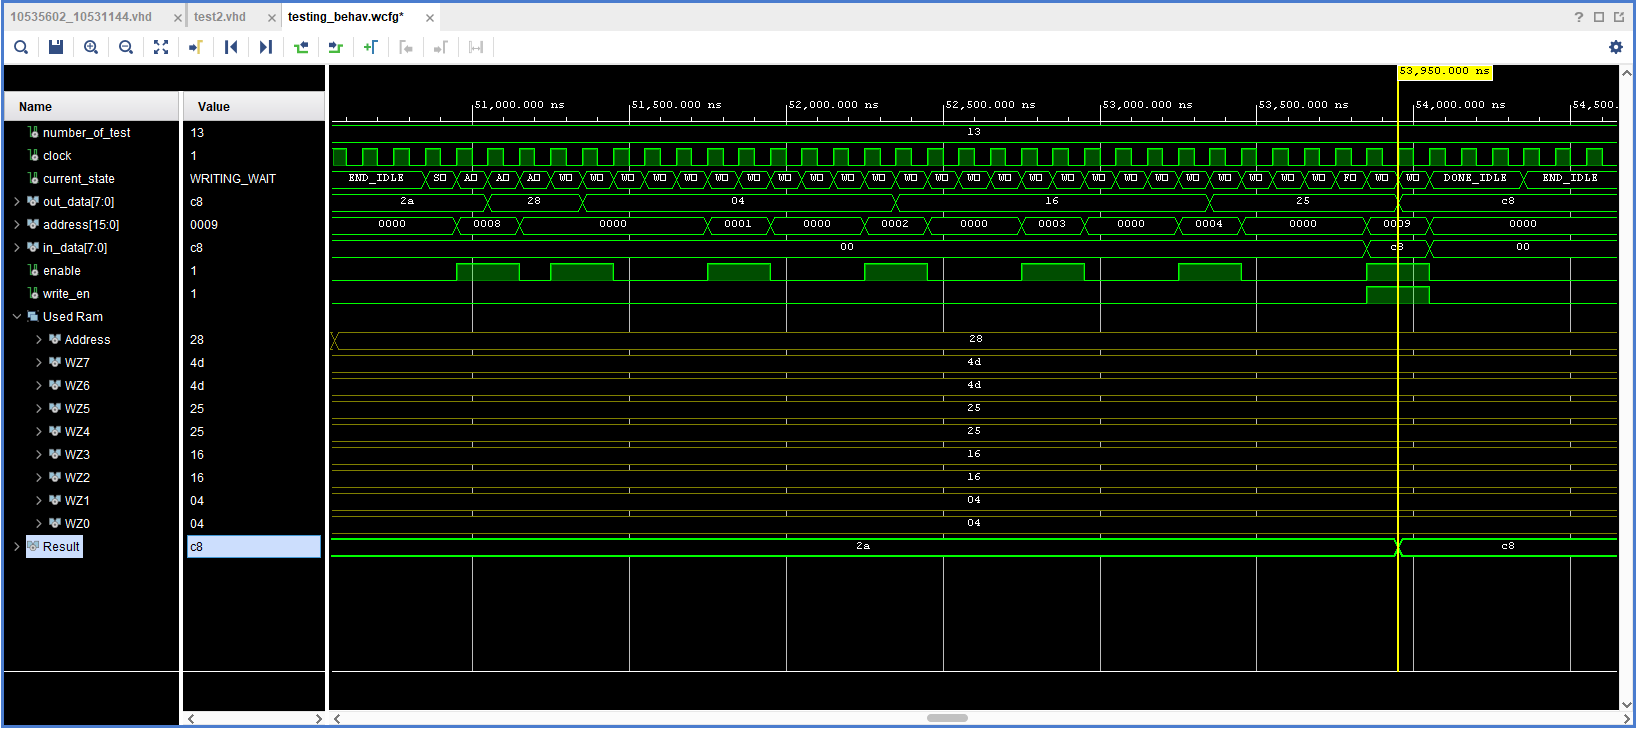
\includegraphics[scale=0.4]{test13.png}
		\end{center}
		\vspace{0.5cm}
	
	\end{enumerate}
		
	\section{Limitazioni e possibili ottimizzazioni}
		\subsection{Scalabilità del componente}
			La specifica fornisce una RAM contenente 8 indirizzi relativi ad altrettante working zone. Il contatore \textit{\texttt{wz\_counter}} è però un contatore a 16 bit, per un migliore collegamento con il segnale d'uscita \textit{\texttt{o\_address}} senza avere valori di tale uscita forzati al valore $0$. La macchina potrebbe essere quindi riadattata per un numero di working zone ben superiore a 8, ma sarebbe comunque necessaria una modifica allo standard di codifica dei risultati ottenuti, ad opera degli stati \textit{\texttt{FOUND\_WZ\_ENCODING}} e \textit{\texttt{NO\_WZ\_ENCODING}}, di fatto legati alla specifica di 8 sole working zone.
		\subsection{Segnale di reset} \label{sec:reset}
			Dal momento che la specifica non riporta alcun vincolo né assunzione sul segnale di reset \textit{\texttt{i\_rst}} e sulla sua durata, abbiamo deciso di sincronizzare la procedura di reset. In particolare, la macchina è in grado di riconoscere una richiesta di reset a prescindere da quanto a lungo il segnale \textit{\texttt{i\_rst}} è rimasto al valore logico $1$, ma deve passare un intero ciclo di clock perché tale reset avvenga. Garantiamo comunque un comportamento coerente con la richiesta di reset: in particolare, non è possibile per la macchina notificare alla RAM la fine dell'elaborazione tramite il segnale \textit{\texttt{o\_done}} nei cicli immediatamente successivi all'innalzamento di \textit{\texttt{i\_rst}}.
		\subsection{Ottimizzazione dei dati nella RAM} \label{sec:ottimizzazione}
			La macchina è progettata per fornire il risultato corretto anche se gli indirizzi relativi alle working zone contenuti nella RAM non sono in ordine $($vedasi la sezione \hyperref[sec:test]{\textit{3: Test eseguiti}}$)$.
			La macchina infatti esegue una scansione lineare di tutte le working zone, decidendo per ogni working zone letta se richiedere la working zone successiva o fermarsi. Perciò, tra tutte le possibili configurazioni, il caso pessimo è quello in cui l'indirizzo base non appartiene a nessuna working zone, oppure quello in cui il base address appartiene alla working zone codificata in \textit{\texttt{RAM($7$)}}.
			Tuttavia, se venisse garantito che gli indirizzi delle working zone nella RAM siano in ordine crescente (o decrescente), sarebbero possibili due modifiche:
			\begin{itemize}
			
			\item \textit{Riduzione dei casi pessimi}: se l'indirizzo della working zone appena esaminata ha un valore più alto dell'indirizzo base, si può concludere che l'indirizzo base non appartiene a nessuna working zone, riducendo così il numero dei casi pessimi. Tale modifica al progetto è piuttosto modesta, dal momento che basterebbe modificare lo stato di \textit{\texttt{WZ\_DECISION}}.
			
			\item \textit{Ricerca binaria}: anziché eseguire una ricerca lineare della working zone risulterebbe più efficiente eseguire una ricerca binaria. Tale strategia ridurrebbe l'intera complessità temporale asintotica della macchina: se $n$ fosse il numero di working zone, si passerebbe da $T(n) \in \mathcal{O}(n)$ a $T(n) \in \mathcal{O}(\log n)$. Tuttavia, questa modifica è più onerosa di quella del punto precedente, dal momento che richiederebbe una modifica all'attuale metodo di scansione (affidato al semplice contatore di working zone \textit{\texttt{wz\_counter}}) e almeno un nuovo stato per il calcolo del prossimo indirizzo di memoria da richiedere.
			\end{itemize}
		\section{Conclusioni}
			Questo componente non ha la pretesa di essere esaustivo in termini di prestazioni. Gli stessi ragionamenti del capitolo precedente porterebbero miglioramenti significativi solo con qualche ipotesi in più, ad esempio supponendo che la memorizzazione delle working zone sia effettivamente ordinabile. Si tratta quindi di speculazioni dipendenti dal contesto in cui opera questo componente, ma esse esulano dallo scopo di questa prova finale.\\
			È importante osservare che, oltre a essere sintetizzabile, il componente descritto è implementabile e supera correttamente entrambe le simulazioni post-implementazione, sia funzionale che temporale. I punti di forza del componente sono legati alla stesura del codice: gli sforzi fatti si sono concentrati sull'evitare bad-practise, fornire un programma leggibile, eliminare ogni warning e fornire una documentazione adeguata, con la forma mentis che contraddistingue l'ingegneria del software.

\end{document}